\documentclass[]{tufte-book}

% ams
\usepackage{amssymb,amsmath}

\usepackage{ifxetex,ifluatex}
\usepackage{fixltx2e} % provides \textsubscript
\ifnum 0\ifxetex 1\fi\ifluatex 1\fi=0 % if pdftex
  \usepackage[T1]{fontenc}
  \usepackage[utf8]{inputenc}
\else % if luatex or xelatex
  \makeatletter
  \@ifpackageloaded{fontspec}{}{\usepackage{fontspec}}
  \makeatother
  \defaultfontfeatures{Ligatures=TeX,Scale=MatchLowercase}
  \makeatletter
  \@ifpackageloaded{soul}{
     \renewcommand\allcapsspacing[1]{{\addfontfeature{LetterSpace=15}#1}}
     \renewcommand\smallcapsspacing[1]{{\addfontfeature{LetterSpace=10}#1}}
   }{}
  \makeatother
\fi

% graphix
\usepackage{graphicx}
\setkeys{Gin}{width=\linewidth,totalheight=\textheight,keepaspectratio}

% booktabs
\usepackage{booktabs}

% url
\usepackage{url}

% hyperref
\usepackage{hyperref}

% units.
\usepackage{units}


\setcounter{secnumdepth}{2}

% citations
\usepackage{natbib}
\bibliographystyle{apalike}
%\renewcommand{\bibsection}{\chapter*{References}}

% pandoc syntax highlighting
\usepackage{color}
\usepackage{fancyvrb}
\newcommand{\VerbBar}{|}
\newcommand{\VERB}{\Verb[commandchars=\\\{\}]}
\DefineVerbatimEnvironment{Highlighting}{Verbatim}{commandchars=\\\{\}}
% Add ',fontsize=\small' for more characters per line
\usepackage{framed}
\definecolor{shadecolor}{RGB}{248,248,248}
\newenvironment{Shaded}{\begin{snugshade}}{\end{snugshade}}
\newcommand{\KeywordTok}[1]{\textcolor[rgb]{0.13,0.29,0.53}{\textbf{{#1}}}}
\newcommand{\DataTypeTok}[1]{\textcolor[rgb]{0.13,0.29,0.53}{{#1}}}
\newcommand{\DecValTok}[1]{\textcolor[rgb]{0.00,0.00,0.81}{{#1}}}
\newcommand{\BaseNTok}[1]{\textcolor[rgb]{0.00,0.00,0.81}{{#1}}}
\newcommand{\FloatTok}[1]{\textcolor[rgb]{0.00,0.00,0.81}{{#1}}}
\newcommand{\ConstantTok}[1]{\textcolor[rgb]{0.00,0.00,0.00}{{#1}}}
\newcommand{\CharTok}[1]{\textcolor[rgb]{0.31,0.60,0.02}{{#1}}}
\newcommand{\SpecialCharTok}[1]{\textcolor[rgb]{0.00,0.00,0.00}{{#1}}}
\newcommand{\StringTok}[1]{\textcolor[rgb]{0.31,0.60,0.02}{{#1}}}
\newcommand{\VerbatimStringTok}[1]{\textcolor[rgb]{0.31,0.60,0.02}{{#1}}}
\newcommand{\SpecialStringTok}[1]{\textcolor[rgb]{0.31,0.60,0.02}{{#1}}}
\newcommand{\ImportTok}[1]{{#1}}
\newcommand{\CommentTok}[1]{\textcolor[rgb]{0.56,0.35,0.01}{\textit{{#1}}}}
\newcommand{\DocumentationTok}[1]{\textcolor[rgb]{0.56,0.35,0.01}{\textbf{\textit{{#1}}}}}
\newcommand{\AnnotationTok}[1]{\textcolor[rgb]{0.56,0.35,0.01}{\textbf{\textit{{#1}}}}}
\newcommand{\CommentVarTok}[1]{\textcolor[rgb]{0.56,0.35,0.01}{\textbf{\textit{{#1}}}}}
\newcommand{\OtherTok}[1]{\textcolor[rgb]{0.56,0.35,0.01}{{#1}}}
\newcommand{\FunctionTok}[1]{\textcolor[rgb]{0.00,0.00,0.00}{{#1}}}
\newcommand{\VariableTok}[1]{\textcolor[rgb]{0.00,0.00,0.00}{{#1}}}
\newcommand{\ControlFlowTok}[1]{\textcolor[rgb]{0.13,0.29,0.53}{\textbf{{#1}}}}
\newcommand{\OperatorTok}[1]{\textcolor[rgb]{0.81,0.36,0.00}{\textbf{{#1}}}}
\newcommand{\BuiltInTok}[1]{{#1}}
\newcommand{\ExtensionTok}[1]{{#1}}
\newcommand{\PreprocessorTok}[1]{\textcolor[rgb]{0.56,0.35,0.01}{\textit{{#1}}}}
\newcommand{\AttributeTok}[1]{\textcolor[rgb]{0.77,0.63,0.00}{{#1}}}
\newcommand{\RegionMarkerTok}[1]{{#1}}
\newcommand{\InformationTok}[1]{\textcolor[rgb]{0.56,0.35,0.01}{\textbf{\textit{{#1}}}}}
\newcommand{\WarningTok}[1]{\textcolor[rgb]{0.56,0.35,0.01}{\textbf{\textit{{#1}}}}}
\newcommand{\AlertTok}[1]{\textcolor[rgb]{0.94,0.16,0.16}{{#1}}}
\newcommand{\ErrorTok}[1]{\textcolor[rgb]{0.64,0.00,0.00}{\textbf{{#1}}}}
\newcommand{\NormalTok}[1]{{#1}}

% longtable
\usepackage{longtable,booktabs}

% multiplecol
\usepackage{multicol}

% strikeout
\usepackage[normalem]{ulem}

% morefloats
\usepackage{morefloats}

% force floats added by CII
\usepackage{float}
\floatplacement{figure}{H}


% tightlist macro required by pandoc >= 1.14
\providecommand{\tightlist}{%
  \setlength{\itemsep}{0pt}\setlength{\parskip}{0pt}}

% title / author / date
\title{LeaRning R in ChemistRy at Reed College}

\author{Chester Ismay}
\date{2016-10-14}

\usepackage{booktabs}
\usepackage{longtable}
\usepackage{framed,color}
\usepackage{float}
\floatplacement{figure}{H}
\usepackage[parfill]{parskip}
\definecolor{shadecolor}{RGB}{248,248,248}

\ifxetex
  \usepackage{letltxmacro}
  \setlength{\XeTeXLinkMargin}{1pt}
  \LetLtxMacro\SavedIncludeGraphics\includegraphics
  \def\includegraphics#1#{% #1 catches optional stuff (star/opt. arg.)
    \IncludeGraphicsAux{#1}%
  }%
  \newcommand*{\IncludeGraphicsAux}[2]{%
    \XeTeXLinkBox{%
      \SavedIncludeGraphics#1{#2}%
    }%
  }%
\fi

%% Need to clean up
\newenvironment{rmdblock}[1]
  {\begin{shaded*}
  \begin{itemize}
  \renewcommand{\labelitemi}{
    \raisebox{-.7\height}[0pt][0pt]{
  %    {\setkeys{Gin}{width=3em,keepaspectratio}\includegraphics{images/#1}}
    }
  }
  \item
  }
  {
  \end{itemize}
  \end{shaded*}
  }
%% Probably can be omitted
\newenvironment{rmdnote}
  {\begin{rmdblock}{note}}
  {\end{rmdblock}}
\newenvironment{rmdcaution}
  {\begin{rmdblock}{caution}}
  {\end{rmdblock}}
\newenvironment{rmdimportant}
  {\begin{rmdblock}{important}}
  {\end{rmdblock}}
\newenvironment{rmdtip}
  {\begin{rmdblock}{tip}}
  {\end{rmdblock}}
\newenvironment{rmdwarning}
  {\begin{rmdblock}{warning}}
  {\end{rmdblock}}
\newenvironment{learncheck}
  {\begin{rmdblock}{warning}}
  {\end{rmdblock}}
\newenvironment{review}
  {\begin{rmdblock}{warning}}
  {\end{rmdblock}}

% To tweak tufte layout
\geometry{
  left=0.8in, % left margin
  textwidth=35pc, % main text block
  marginparsep=1pc, % gutter between main text block and margin notes
  marginparwidth=8pc % width of margin notes
}

\begin{document}

%\let\allcaps=\relax
\maketitle



{
\setcounter{tocdepth}{1}
\tableofcontents
}

\chapter*{Introduction}\label{introduction}
\addcontentsline{toc}{chapter}{Introduction}

\section*{What is this?}\label{what-is-this}
\addcontentsline{toc}{section}{What is this?}

In the HTML version of this book, you can also download the PDF version
of the book by clicking on PDF button in the top toolbar of the page.
HTML is the preferred format but the PDF format may be preferred for
some readers. Links to the different GIFs directly found in the HTML
version are provided in the PDF version.

This resource is designed to assist students in CHEM 101/102 in using
RStudio and R Markdown to complete their labs. (A more general reference
to the specifics of R, RStudio and R Markdown is available in a
different free book \href{http://ismayc.github.io/rbasics-book}{here}
\citep{usedtor2016}). This resource will show you GIFs explaining how to
do some common procedures you'll need to do to complete labs. In
addition, it will provide more details about the specifics of the
different lab templates available in the \texttt{chemistr} R package.
Each chapter of this book will correspond to each of the different labs.

Lastly, if you are interested, you'll find instructions on how to
complete the labs using RStudio Desktop instead of the RStudio Server in
the Appendix. The Appendix will also include descriptions of the code
that is sitting ``behind the scenes'' in many of the functions created
in the \texttt{chemistr} package: \texttt{chem\_table},
\texttt{chem\_scatter}, \texttt{chem\_clustered.bar}, etc. These
functions were written to ease a beginner into working with R. Those
interested in customizing their lab reports further should look over the
R code in the Appendix. Additionally, many of the needed packages are
automatically loaded when the \texttt{chemistr} package is loaded using
\texttt{library(chemistr)}. You'll see how each of these packages is
used in the Appendix.

If further clarification is needed on any other aspect of the book,
please email \href{mailto:cismay@reed.edu}{me} with a reference to the
error/area where more guidance is necessary. More advanced users are
encouraged to create a GitHub issue
\href{https://github.com/ismayc/chemistr-book/issues}{here}. Pull
requests on GitHub for typos or improvements are also welcome and you
can easily do so by clicking on the Edit button near Search at the top
of the HTML version of the book.

This book will evolve and be updated as needed based on feedback. You
can always check the date at the end of the chapter to see when the book
was last updated. It is recommended that you use Google Chrome as your
browser since GIFs sometimes do not load automatically with other
browsers.

\section*{Starting the labs}\label{starting-the-labs}
\addcontentsline{toc}{section}{Starting the labs}

\subsection*{Logging in and initial
screen}\label{logging-in-and-initial-screen}
\addcontentsline{toc}{subsection}{Logging in and initial screen}

The RStudio Server provides a web-based way to run analyses in R. This
means that you will only need an internet connection and a web browser
to run your analyses. You can be running a Windows machine, a Mac, a
Linux, or pretty much any other device that has access to the internet
and a web browser. If you are interested in using the Reed College
RStudio Server off campus, you'll need to request access in the form
\href{https://docs.google.com/a/reed.edu/forms/d/e/1FAIpQLSftEFv1v-GAwrH4fy-eIoToHBybWyXRSJUwk-NKHU6-Gn5Q6g/viewform}{here}.
The initial login page will not load for you unless you are connected to
the VPN from off campus locations. After entering the link
(\url{http://rstudio-dev.reed.edu}) into your browser, you'll see a page
that looks something like:

\begin{center}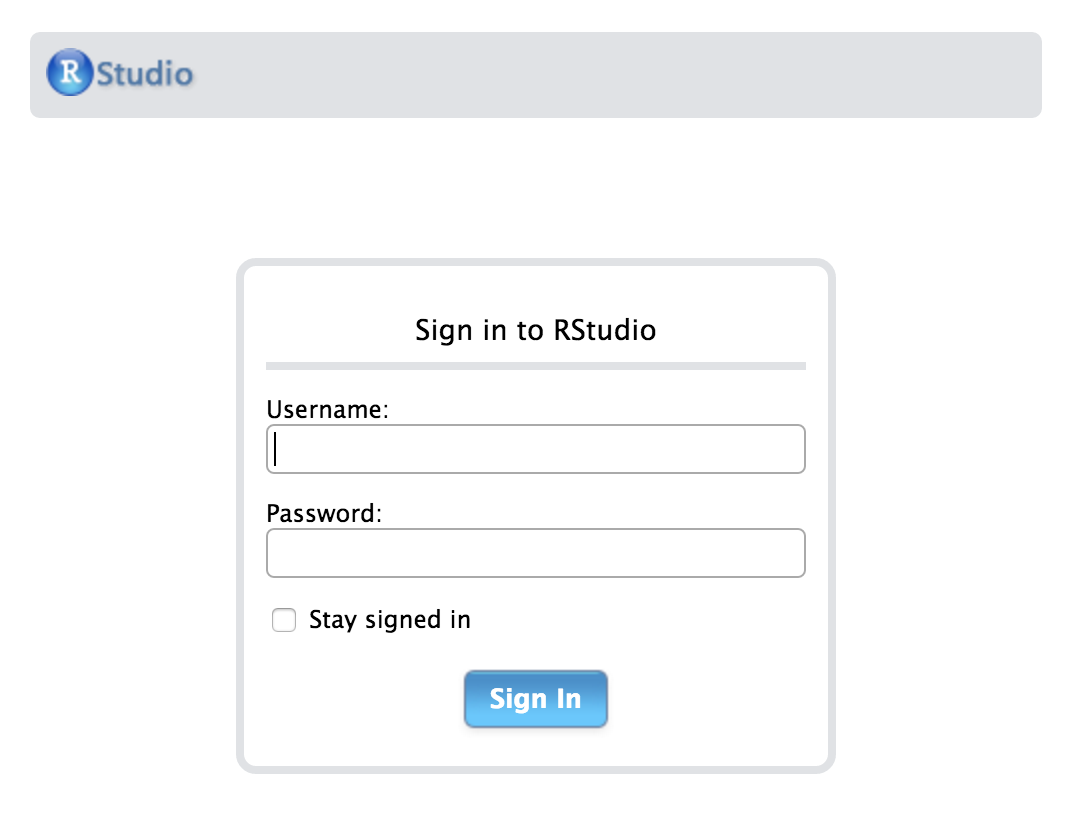
\includegraphics[width=0.5\linewidth]{screenshots/server_login} \end{center}

After logging in with your Reed College username (mine is
\texttt{cismay}, for example) and password, you should see a layout
similar to what follows.

\begin{center}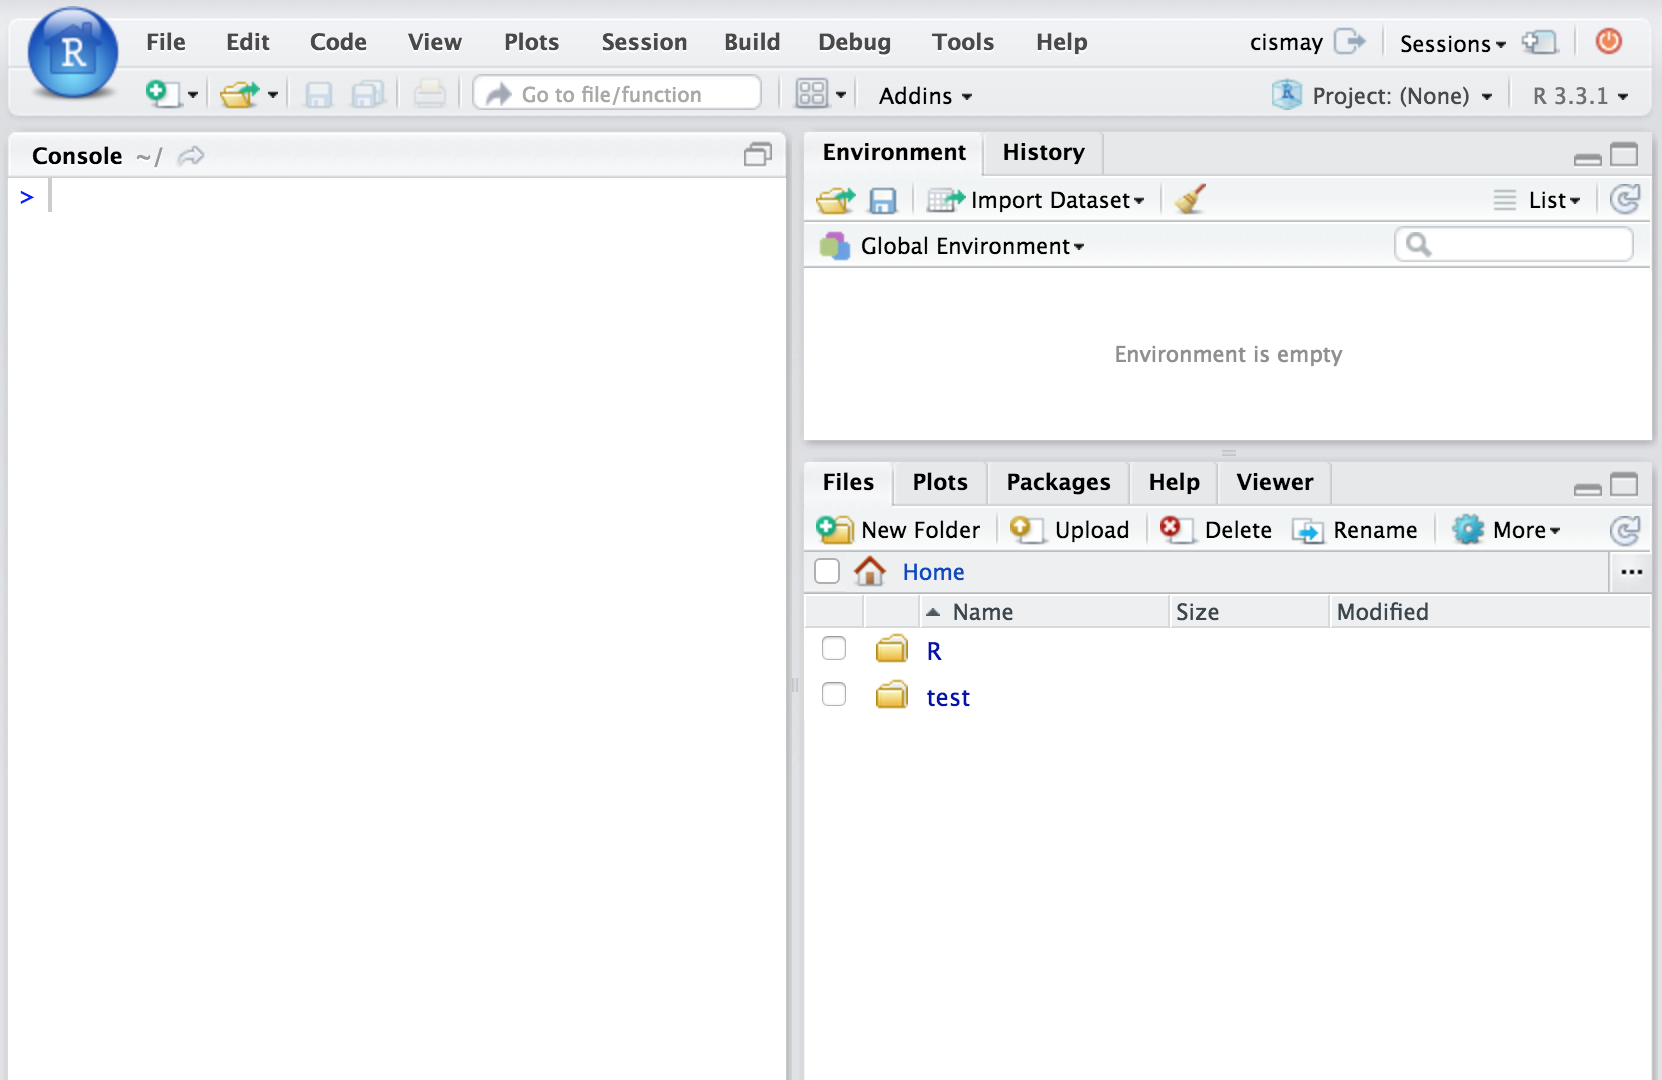
\includegraphics[width=0.7\linewidth]{screenshots/initial_rstudio} \end{center}

\subsection*{Creating and Sharing Projects using RStudio
Server}\label{creating-and-sharing-projects-using-rstudio-server}
\addcontentsline{toc}{subsection}{Creating and Sharing Projects using
RStudio Server}

A good habit to get into whenever you start a new project following a
common theme (such as your CHEM 101 labs) with R code is to create a new
RStudio project to go along with it. RStudio project files have the
extension \texttt{.Rproj} and store metadata that goes along with the
documents you've saved and information about the R environment you are
working in. More information about RStudio projects is available from
RStudio, Inc.
\href{https://support.rstudio.com/hc/en-us/articles/200526207-Using-Projects}{here}.

You'll be sharing your Chem 101 labs with your Danielle Cass
(\texttt{dcass}) and Chester Ismay (\texttt{cismay}) using the RStudio
Server. This will allow both of us to help you with errors you may be
having in writing your lab report without having to email files back and
forth. You'll just need to email us with the name of the lab you are
having troubles with and what you named your RStudio project and we'll
be able to go in and look over your R Markdown file. You can think of
this as working somewhat like Google Docs in that both Danielle and I
can provide feedback and walk-through your analyses.

To share the project with us, you should follow along with the example
below. Instead of naming your RStudio project
\texttt{CHEM101\_ChesterIsmay} as the GIF shows, you should name it
\texttt{CHEM101\_YourName} where \texttt{YourName} is replaced with your
first and last names. Spaces can cause problems in file names so it is
recommended that you avoid them. If you've already shared your project
and you have spaces in the name, you'll probably be OK, but try to avoid
spaces in your file names going forward. Calling your project
\texttt{CHEM101\_YourName} will allow Danielle and I to track down your
project more easily than if everyone named their project
\texttt{initial} or something similar.

\vspace{0.1in}

\begin{center}\footnotesize{\url{https://raw.githubusercontent.com/ismayc/chemistr-book/master/gifs/proj_share.gif}}\end{center}

\vspace{0.1in}

You'll need to also add \texttt{cismay} as someone you'd like to share
the project with. You can do so by entering my username immediately
after you have clicked \textbf{Add} to add Danielle or you can go back
to \textbf{Share Project} and enter my name there just as you have with
\texttt{dcass}. If you see that your project is shared with both
\texttt{dcass} and \texttt{cismay}, you have completed this stage
successfully.

You'll see at the beginning of each chapter corresponding to the labs
how you can access the different R Markdown template files for each lab.
These template files are built into the \texttt{chemistr} package that I
have already loaded on the Reed RStudio Server for you. \footnote{If you
  are completing the labs using RStudio Desktop, you'll see instructions
  on how to install this package onto your computer in the Appendix.
  After installing the package, you'll be able to use the R Markdown
  templates in much the same way students using the RStudio Server can.
  Note that if you are using the RStudio Desktop, you won't have access
  to the Shared Projects feature and it will be more difficult for
  Danielle and I to help you.}

\subsection*{Don't overwrite the Rproj
file!}\label{dont-overwrite-the-rproj-file}
\addcontentsline{toc}{subsection}{Don't overwrite the Rproj file!}

\textbf{Important Note}: There is a BIG difference between an Rmd (R
Markdown) file that will store the code for each of your labs and this
Rproj (RStudio Project) file. \textbf{DO NOT OVERWRITE the Rproj file
with your Rmd file or any other file}. If you do this, Danielle and I
will not be able to assist you since the Rproj file stores important
information about sharing projects. You'll need to create a new project
all over from the beginning and it's much better for everyone to not
overwrite this file. Please create a new folder for each lab and
\textbf{LEAVE THIS Rproj file ALONE}.

\section*{Requesting help}\label{requesting-help}
\addcontentsline{toc}{section}{Requesting help}

It's nearly impossible for Danielle and I to help you unless we know
that you are having troubles. If you find yourself unable to complete a
lab because of problems with RStudio and you've spent more than 30
minutes trying to figure it out, it is time for you to stop and ask for
help. We encourage you to try to figure it out on your own as much as
possible because this helps you learn, but if you are deeply entrenched
in not getting R to work, that could be taking away from your learning
of Chem 101/102 material.

We encourage you to reach out to both of us and carefully explain what
is going wrong with your R Markdown file. Sending us an email saying ``I
can't get it to work, please help.'' is not insightful and won't help
you learn in the long-run. Be as descriptive as possible. Something like
what follows is much preferred:

\vspace{0.1in}

\begin{quote}
``I'm receiving an error on line 46 of my Light lab about not finding an
object. I've tried Googling it and found a couple references about it
including \textbf{link1} and \textbf{link2} but it's not working for
me.''
\end{quote}

\vspace{0.1in}

This tells us that you have tried to figure it out for yourself, but
that you require our assistance. That is to be expected and you
shouldn't be discouraged if you don't understand something about R
Markdown immediately.

We are here to help and please don't give up on this. Learning how to
work with R even at the most basic of levels will help you long-term in
keeping track of analyses and getting you on the path to reproducible
research. This will help you in your academic careers and whatever you
do after your academic career ends. If you need assistance, please email
\href{dcass@reed.edu}{Danielle} and \href{cismay@reed.edu}{Chester} with
your concise error specifying in which lab and what the name of your
RStudio project is. We are happy to help you learn how to use R!

Additionally, it is extremely helpful for us if you can share a link to
your RStudio Project in any emails requesting help. This link is
available by going to your RStudio project in the top right corner of
RStudio, clicking on it and then selecting \textbf{Share Project}, and
then select \textbf{Sharing} as seen in the screenshots below.

\begin{center}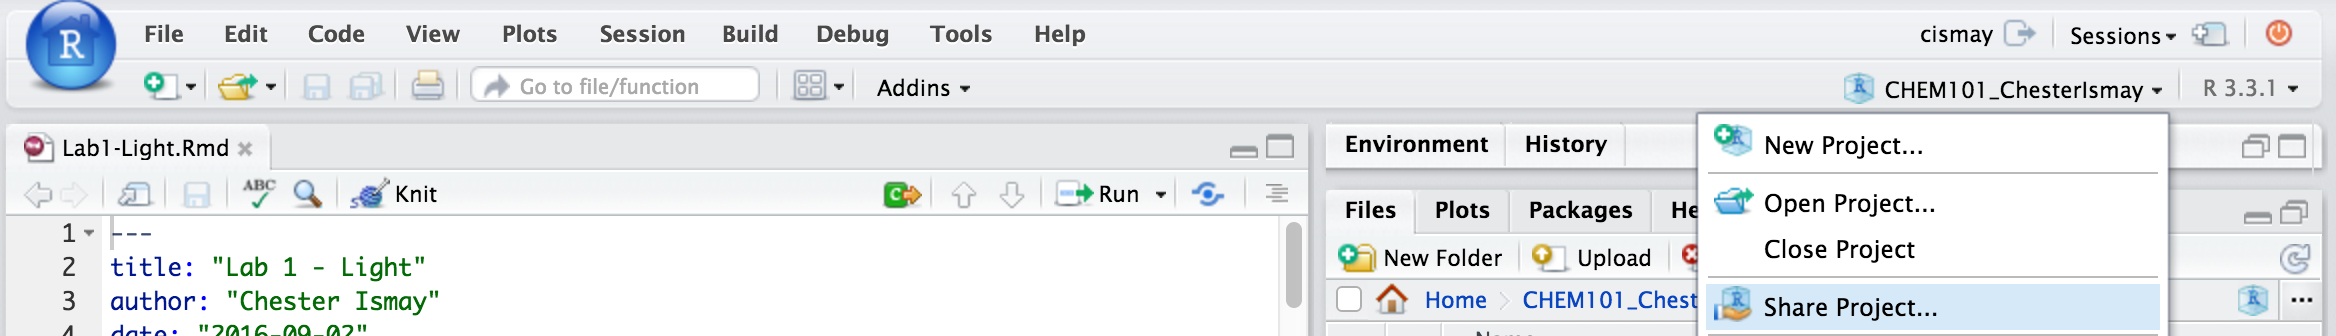
\includegraphics[width=\textwidth]{screenshots/shareproj1} \end{center}

\begin{center}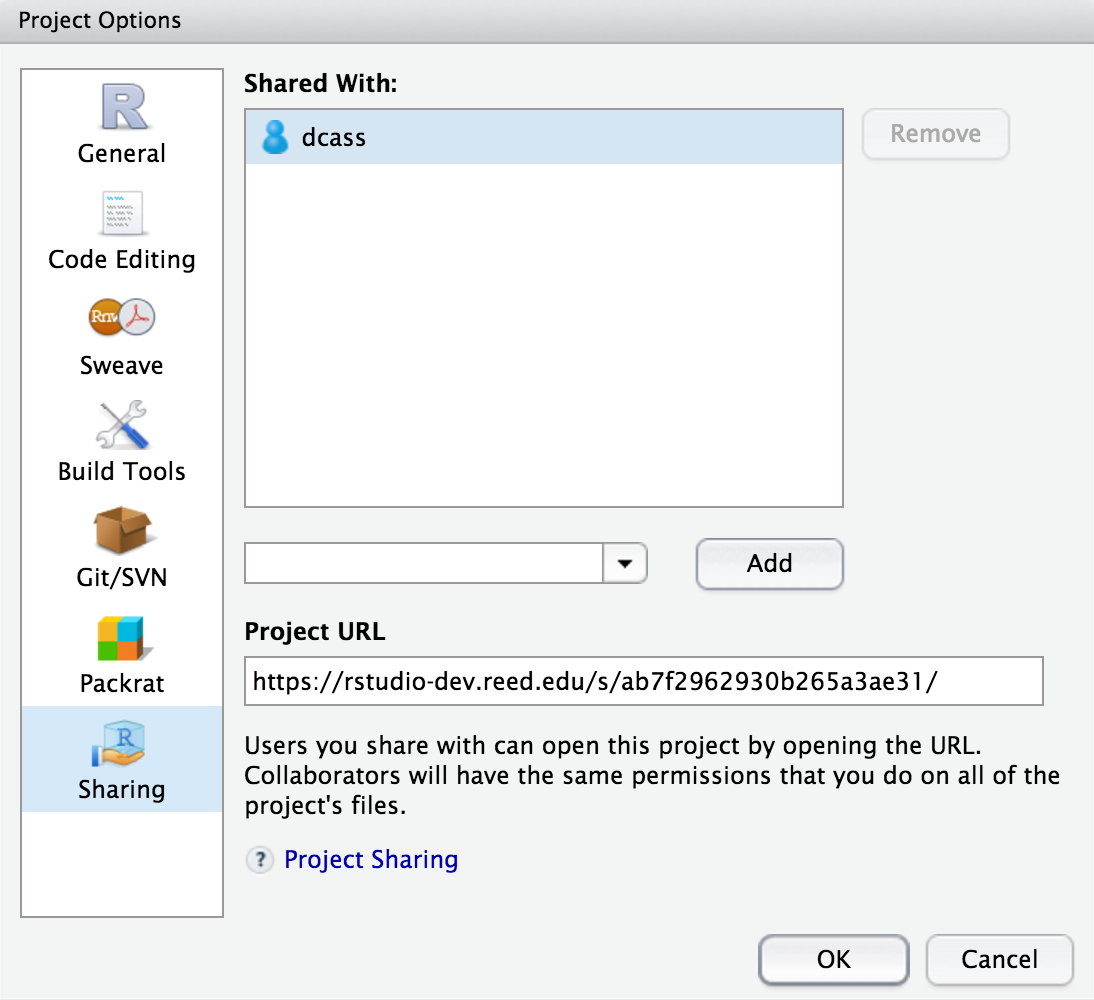
\includegraphics[width=0.6\linewidth]{screenshots/shareproj2} \end{center}

The link is given in the \textbf{Project URL}. Please copy this entire
link into the body of your emails to Danielle or I so that we can
quickly look into your errors.

\subsection*{Book was last updated:}\label{book-was-last-updated}
\addcontentsline{toc}{subsection}{Book was last updated:}

\begin{verbatim}
## [1] "By cismay on Friday, October 14, 2016 17:21:35 PDT"
\end{verbatim}

\chapter{Lab 1: Light}\label{light}

\hypertarget{getting-the-lab-template}{\section{Getting the lab
template}\label{getting-the-lab-template}}

In RStudio, you'll find the R Markdown template that you will update
with your own results by following along with the GIF below:

\vspace{0.1in}

\begin{center}\footnotesize{\url{https://raw.githubusercontent.com/ismayc/chemistr-book/master/gifs/light_template.gif}}\end{center}

\vspace{0.1in}

I've also created a new folder called \texttt{Lab1-Light} in my
\texttt{CHEM101\_ChesterIsmay} folder and named the resulting R Markdown
file that was loaded in from the R Markdown template in
\texttt{chemistr} the same thing: \texttt{Lab1-Light.Rmd}. You are
highly encouraged to follow this same convention for all of your labs.
(Note that as I mentioned earlier in this manual I do not have any
spaces in the folder names or in the names of files here.) This will
allow you to remember exactly where you stored the files and allow
Danielle and I to easily find your files on the RStudio Server. Note
that this folder was also created in the \texttt{CHEM101\_ChesterIsmay}
folder where the \texttt{Rproj} file resides. If you put your lab in the
\texttt{Home} directory instead, Danielle and I won't be able to access
it since \texttt{Home} is the parent directory of
\texttt{CHEM101\_YourName}.

\section{The parts of the lab
template}\label{the-parts-of-the-lab-template}

\hypertarget{the-yaml-header}{\subsection{The YAML
header}\label{the-yaml-header}}

I've already entered some values into my R Markdown file. First I gave a
title to the R Markdown file: ``Lab 1 - Light''. I then entered my name
and the current date. All of these are in quotation marks since they all
correspond to character strings and not numbers. It will likely still
work if you don't put quotation marks around the entries here, but it is
recommended that you use the quotation marks to help you understand the
use of quotation marks when you begin working with R code. (R won't be
as nice as YAML is on forgetting quotation marks when they are needed.)

This portion of the R Markdown file is called the YAML header. It stores
metadata about your document. It is separated by \texttt{-\/-\/-} before
and \texttt{-\/-\/-} after on their own lines. RStudio will warn you by
coloring the \texttt{-\/-\/-} red if you accidentally add a space before
them.

You'll need to make sure to include a space after each of the YAML
entries. You'll receive an error if you have something like that below,
for example:

\begin{Shaded}
\begin{Highlighting}[]
\FunctionTok{title:} \StringTok{"Light Lab"}
\FunctionTok{author:} \StringTok{"Chester Ismay"}
\FunctionTok{date:}\StringTok{"August 30, 2016"}
\FunctionTok{output:} \NormalTok{chemistr::chem_lab_word}
\end{Highlighting}
\end{Shaded}

There needs to be a space after the \texttt{:} for the \texttt{date}
field.

The last line here corresponds to the type of output that will be
produced. In this case, I've created a nice way for you to output this R
Markdown file to a DOCX (Word document) format. The
\texttt{chem\_lab\_word} document format in \texttt{chemistr} creates a
Word document with figure captions enabled by default and images with
size 3 inches in height and 6 inches in width by default.

\subsection{Initial R Chunk}\label{initial-r-chunk}

On line 8 of the Light R Markdown template, you'll see three backticks
starting the line. This tells R Markdown to expect a block/chunk of
code. This code is R code by the next designation \texttt{\{r}. Next we
give this R chunk a name \texttt{setup} and then specify chunk options
immediately after the name and a comma. Here we have specified
\texttt{include=FALSE}. We then close the specifications for the chunk
with a \texttt{\}}. This \texttt{include=FALSE} chunk option will run
the R code when we press \textbf{Knit} button near the top of the code
editor will not put the R code or its output into the document. We'll
press the \textbf{Knit} button in a bit to understand what it
accomplishes.

You'll see this \texttt{setup} chunk in all of the lab templates. It's
good practice to load any package you'll need for your analysis at the
top in a chunk like this. You may not initially understand why
\texttt{chemistr} is needed but it will be needed when we create a table
using the \texttt{chem\_table} function, which resides in the
\texttt{chemistr} package, in the \texttt{table} chunk beginning on line
21.

\subsection{Headers}\label{headers}

Immediately below this first R chunk is two hash tags. This corresponds
to creating a header in our resulting document. The font immediately
following the hash-tags will be larger and act as a divider in our
document. The number of hash-tags you enter corresponds to how large
you'd like to make the header. One hash-tag is the largest and six is
the smallest. It is recommended that you use between one and three
hash-tags for headers.

\subsection{Enter data chunk}\label{enter-data-chunk}

If you press the \textbf{Knit} button at this moment, you'll receive an
error. Let's look into what this error means:

\vspace{0.1in}

\begin{center}\footnotesize{\url{https://raw.githubusercontent.com/ismayc/chemistr-book/master/gifs/knit_error1.gif}}\end{center}

\vspace{0.1in}

Danielle has created lab templates that might not necessarily build
without errors immediately for you. You should carefully read over the
directions in each chunk (The comments after the \texttt{\#} in the R
chunks.) before pressing \textbf{Knit}. Here we see that the error
occurs near line 15 of our R Markdown file. The \texttt{Color} and
\texttt{WavelengthRange} vectors need to have some values entered. These
results will correspond to what you observed in lab. I will enter some
demo results in here and also show you how to use the R Console to check
your results. You'll see that the \texttt{Color} and
\texttt{WavelengthRange} vectors must be of the same length when we
create a \texttt{data\_frame} to combine them together into
``spreadsheet'' format in the variable named \texttt{Q1\_data}:

\vspace{0.1in}

\begin{center}\footnotesize{\url{https://raw.githubusercontent.com/ismayc/chemistr-book/master/gifs/enter_data_full.gif}}\end{center}

\vspace{0.1in}

You should use the R Console to check your results in the R chunks by
either entering the R code line by line into the Console or by pressing
the \textbf{Run Current Chunk} button (the green Play button). We see
here that \texttt{Q1\_data} is 6 rows by 2 columns and stores our
results in ``spreadsheet'' form as a \texttt{data\_frame}.

Note that you'll also receive an error if you have a different number of
entries for \texttt{WavelengthRange} and \texttt{Color}. Data frames
must have an equal number of rows when you combine the columns together
via \texttt{data\_frame}.

The \texttt{chemistr} package also loads the \texttt{dplyr} package
where the \texttt{data\_frame} function resides. If you are running the
chunks by pressing the green ``play'' button, which sends the current
chunk into the R console, you'll need to remember to load all previous
chunks as well. If you receive an error message such as

\begin{verbatim}
Error: could not find function "data_frame"
\end{verbatim}

this means that you have not loaded the \texttt{chemistr} package by
sending the \texttt{library(chemistr)} code into the Console BEFORE you
run the declarations for \texttt{Color}, \texttt{Wavelength}, and
\texttt{Q1\_data\ \textless{}-\ data\_frame(Color,\ WavelengthRange)}.
The code chunks read like a book so if you are receiving errors of the
``could not find'' variety, it probably means you haven't run all chunks
up to the point of your current chunk in the Console. These sorts of
errors are also referenced in Chapter 6 of ``Getting Used to R, RStudio,
and R Markdown''\citep{usedtor2016}.

\subsection{A nice table R chunk}\label{a-nice-table-r-chunk}

The \texttt{chem\_table} function will result in a nicely formatted
table being produced in your resulting Word document. You'll need to
specify a caption inside the parentheses instead of the
\texttt{"A\ lovely\ caption\ for\ the\ table"} default. You'll also see
that RStudio will create a second quotation mark when you might not want
one. Carefully look over your document if you have errors and make sure
there aren't two quotation marks when you only wanted one. You'll see
this below:

\vspace{0.1in}

\begin{center}\footnotesize{\url{https://raw.githubusercontent.com/ismayc/chemistr-book/master/gifs/two_quotes.gif}}\end{center}

\vspace{0.1in}

After fixing our error, we have now created a DOCX file that will have
our nice table showing the \texttt{Q1\_data}. Feel free to open up this
\texttt{Lab1\_Light.docx} file now and see that the table was created
with the caption ``Light Source Table''. You should probably enter a
different and more specific caption instead though.

If you scroll down the R Markdown file, you'll see that there are many
more spots where we will be inserting pictures. R Markdown has nicely
skipped over these chunks when we pressed \textbf{Knit} instead of
halting and giving lots of confusing errors and we see that in the R
Console window under the R Markdown tab.

\section{Uploading and inserting external
pictures}\label{uploading-and-inserting-external-pictures}

You'll frequently be asked to add pictures into your lab reports that
weren't necessarily created using R. (We will see how to include plots
created inside R in later labs though.) If you look over \textbf{Q2} in
the lab it is asking you to include a picture of the ``Absorbance
spectrum of water in a 1 cm cuvette''. Note that this is specified as
the figure caption here for the first R chunk after \textbf{Q2}.

Mathematical text is also included by surrounding the mathematical
expression with dollar signs. This is using LaTeX to produce nicely
formatted math text. Here we see the expression \(H_{2}O\) is given
using \texttt{\$H\_\{2\}O\$}.

In order to include a picture, you'll need to first upload it to the
RStudio Server into the directory where the R Markdown file is located.
The GIF below shows you how to do so. Remember that you'll need to know
where you saved your image on your computer to specify it here. This
example GIF is recorded on a Mac but similar procedures should be done
on a Linux or Windows machine.

\vspace{0.1in}

\begin{center}\footnotesize{\url{https://raw.githubusercontent.com/ismayc/chemistr-book/master/gifs/upload_photo.gif}}\end{center}

\vspace{0.1in}

The \texttt{Water.jpg} file has been uploaded to my \texttt{Lab1-Light}
folder on the RStudio Server. The \texttt{include\_graphics} function
requires that you add the name of the file and its extension here. We
now press the \textbf{Knit} button to see the resulting Word document:

\vspace{0.1in}

\begin{center}\footnotesize{\url{https://raw.githubusercontent.com/ismayc/chemistr-book/master/gifs/knitted.gif}}\end{center}

\vspace{0.1in}

\subsection{The remainder of the lab}\label{the-remainder-of-the-lab}

In the remaining portions of the lab you'll be asked to include other
pictures from your lab sessions and also include a discussion of your
results. This discussion will proceed in much the same way as you would
add a discussion into a Word document or Google Doc. You'll be able to
immediately discuss what occurred in your R chunks right below them.
This allows for the reader to easily follow your work.

\section{Note on white space}\label{note-on-white-space}

As you look over the R Markdown document you'll see that there is always
a new line of white space between the discussion and the R chunks and
also between each of the R chunks. It is highly recommended that you
also follow this workflow. You'll receive some strange errors at times
if you try to stack everything together and it's also much harder to
follow for another reader of your document if you have everything
bunched together. \textbf{White space is your friend!}

\section{Spell-check}\label{spell-check}

Just as I'm sure your English teachers have told you to spell check your
documents before submitting, you are also encouraged to do so here.
There is a built-in spell check option found near the \textbf{Knit}
button.

\begin{center}
\includegraphics[width=0.3\textwidth]{images/spellcheck} \end{center}

Please run this and carefully read over your lab report before
converting it to a PDF and submitting it to Moodle.

\section{Converting your Word document to
PDF}\label{converting-your-word-document-to-pdf}

The directions for each lab on Moodle say to upload a PDF version of
your lab. You'll see how to create this PDF from inside Microsoft Word
for Mac. A similar procedure can be done using LibreOffice
(\url{https://www.libreoffice.org/download/libreoffice-fresh/}) on
Linux, Mac, or Windows machines or Microsoft Word on a PC. You may also
have the option to \textbf{Save As} a PDF there and you can get to this
option by going to \textbf{File -\textgreater{} Save As -\textgreater{}
File Format: -\textgreater{} PDF} on the Mac if you prefer.

\vspace{0.1in}

\begin{center}\footnotesize{\url{https://raw.githubusercontent.com/ismayc/chemistr-book/master/gifs/word_pdf.gif}}\end{center}

\vspace{0.1in}

\hypertarget{beers}{\chapter{Lab 2: Beer's Law}\label{beers}}

\section{Getting the R Markdown lab
template}\label{getting-the-r-markdown-lab-template}

Begin by creating a new folder called \texttt{Lab2-Beers} in your
\texttt{CHEM101\_FirstnameLastname} folder. Next, follow steps similar
to those found in the GIF in
\protect\hyperlink{getting-the-lab-template}{Section 1.1}, but select
the \textbf{Beer's Law} R Markdown template instead of \textbf{Light}
and save your file in the newly created \texttt{Lab2-Beers} folder as
\texttt{lab2.Rmd}.

\section{The parts of the lab
template}\label{the-parts-of-the-lab-template-1}

\subsection{YAML}\label{yaml}

Refer back to \protect\hyperlink{the-yaml-header}{The YAML header}
section in Chapter \ref{light} for a review on what the entries here
mean. Remember to be careful with spacing!

\subsection{Initial R Chunk}\label{initial-r-chunk-1}

Remember that the \texttt{chemistr} package automatically loads in many
useful packages for you. It also includes functions such as
\texttt{chem\_table} you worked with in Lab 1 and \texttt{chem\_scatter}
that you will work with in this lab.

\subsection{Directions chunk}\label{directions-chunk}

Immediately after the \texttt{\#\#\ Data} header, you'll see a chunk of
commented R code Danielle has including giving you directions on what
the chunks after it should include. Note that this chunk again uses
\texttt{include=FALSE} so you won't see any of this in the resulting
knitted DOCX file.

\subsection{First data chunk}\label{first-data-chunk}

After carefully reading over the commented R code Danielle has added
providing you with directions, you now are ready to enter values in for
Part A. Note that you can change the variable names from
\texttt{Independent1} and \texttt{Dependent1} to something else, but
remember that those names cannot include spaces or other mathematical
objects. Remember that if you change the name of \texttt{Independent1}
to, say, \texttt{my\_indep} that you'll need to make sure to change all
references from \texttt{Independent1} to \texttt{my\_indep} in the R
code that follows.

\subsection{Transforming to a logarithmic
scale}\label{transforming-to-a-logarithmic-scale}

We often need to look at data not on our usual scale but instead on a
logarithmic scale. With logarithms we specify a base and you may
remember from algebra that logarithms are related to exponential
functions. To further emphasize this, recall that \(10^2 = 100\) can be
written as \(\log_{10}100 = 2\).

It important to note that \(log_{10}0 = -\infty\) so you'll need to be
careful with how you handle values of 0 when you calculating a
logarithmic function on a vector including 0. For this lab, you are
encouraged to remove any 0 values from your vectors BEFORE you take the
logarithm to avoid this problem.

In this lab, you'll be using ``log base 10'' and the \texttt{log10}
function in R. I recommend you enter \texttt{?log10} into the R Console
for more information on how to do a base 10 logarithmic transformation
on a vector in R. Additionally, you can find a great explanation of how
logarithms are used in the real world
\href{https://betterexplained.com/articles/using-logs-in-the-real-world/}{here}.

One of the powerful features of R is its ability to do vectorized
calculations. Here is an example:

\begin{Shaded}
\begin{Highlighting}[]
\NormalTok{my_nums <-}\StringTok{ }\KeywordTok{c}\NormalTok{(}\DecValTok{10}\NormalTok{, }\DecValTok{15}\NormalTok{, }\DecValTok{105}\NormalTok{, }\DecValTok{500}\NormalTok{, }\DecValTok{100231}\NormalTok{)}
\KeywordTok{log10}\NormalTok{(my_nums)}
\end{Highlighting}
\end{Shaded}

\begin{verbatim}
## [1] 1.000000 1.176091 2.021189 2.698970 5.001002
\end{verbatim}

The code above produces the ``log base 10'' for each of the values in
\texttt{my\_nums}. We haven't assigned this to anything though since we
didn't include the assignment operator \texttt{\textless{}-}. In the GIF
below, I'll show you how to create one of the two new variables you'll
need to create. Remember that you'll also need to update your
\texttt{data\_frame} call to include both of your newly created
variables as well.

\vspace{0.1in}

\begin{center}\footnotesize{\url{https://raw.githubusercontent.com/ismayc/chemistr-book/master/gifs/log.gif}}\end{center}

\vspace{0.1in}

As I have in the GIF, you should use the R Console to check your results
in the R chunks by either entering the R code line by line into the
Console or by pressing the \textbf{Run Current Chunk} button (the green
Play button).

\subsection{Copying from one chunk into a new
chunk}\label{copying-from-one-chunk-into-a-new-chunk}

When you are first learning to program, one of the best strategies you
can do is to copy working code and make small changes to the code to
produce a different result. In the \texttt{plot1} chunk (remember to
look at the phrase right after the \texttt{\{r} and before the comma
that begins your R chunk to find the name), you will see how to produce
a scatterplot of \texttt{Dependent1} on the vertical axis and
\texttt{Independent1} on the horizontal axis (frequently written as ``a
scatterplot of \texttt{Dependent1} versus \texttt{Independent1}---or
\texttt{y} versus \texttt{x}). In the GIF below, you'll see how we could
produce a plot of the log base 10 of \texttt{Dependent1} versus
\texttt{Independent1}. Notice that only a few subtle changes are needed
to produce a different plot. Also think about how the new plot in chunk
\texttt{plot2} compares to the plot produced in \texttt{plot1}.

\vspace{0.1in}

\begin{center}\footnotesize{\url{https://raw.githubusercontent.com/ismayc/chemistr-book/master/gifs/log2.gif}}\end{center}

\vspace{0.1in}

You'll need to use keyboard shortcuts to copy-and-paste code. (Ctrl + C
on a Windows machine or Command + C on a Mac to copy. Then use Ctrl + V
on a Windows machine or Command + V on a Mac to paste.)

\subsection{Regression}\label{regression}

Carefully note in the GIF how I have updated the variables to produce a
new fit and a new plot. The \texttt{lm} function expects
\texttt{y\ \textasciitilde{}\ x} so make sure you have them in the
correct order. In other words, you'll want to have your ``dependent
variable'' \textasciitilde{} ``independent variable''. This is used to
get the coefficients from a straight line regression fit of the data.
The \texttt{summary} function produces a lot of important information
about this fit.

\subsection{The remainder of the lab}\label{the-remainder-of-the-lab-1}

In the remaining portions of the lab, you are asked to modify the
results above to make 4 additional plots. Additionally, you'll need to
provide commentary text below the Discussion header.

\section{Note on white space}\label{note-on-white-space-1}

As you look over the R Markdown document you'll see that there is always
a new line of white space between the discussion and the R chunks and
also between each of the R chunks. It is highly recommended that you
also follow this workflow. You'll receive some strange errors at times
if you try to stack everything together and it's also much harder to
follow for another reader of your document if you have everything
bunched together. \textbf{White space is your friend!}

\section{Spell-check}\label{spell-check-1}

Just as I'm sure your English teachers have told you to spell check your
documents before submitting, you are also encouraged to do so here.
There is a built-in spell check option found near the \textbf{Knit}
button.

\begin{center}
\includegraphics[width=0.3\textwidth]{images/spellcheck} \end{center}

Please run this and carefully read over your lab report before
converting it to a PDF and submitting it to Moodle.

\section{Converting your Word document to
PDF}\label{converting-your-word-document-to-pdf-1}

The directions for each lab on Moodle say to upload a PDF version of
your lab. You'll see how to create this PDF from inside Microsoft Word
for Mac. A similar procedure can be done using LibreOffice
(\url{https://www.libreoffice.org/download/libreoffice-fresh/}) on
Linux, Mac, or Windows machines or Microsoft Word on a PC. You may also
have the option to \textbf{Save As} a PDF there and you can get to this
option by going to \textbf{File -\textgreater{} Save As -\textgreater{}
File Format: -\textgreater{} PDF} on the Mac if you prefer.

\vspace{0.1in}

\begin{center}\footnotesize{\url{https://raw.githubusercontent.com/ismayc/chemistr-book/master/gifs/word_pdf.gif}}\end{center}

\vspace{0.1in}

\section{Note on requesting help}\label{note-on-requesting-help}

It is extremely helpful for us if you can share a link to your RStudio
Project in any emails requesting help. This link is available by going
to your RStudio project in the top right corner of RStudio, clicking on
it and then selecting \textbf{Share Project}, and then select
\textbf{Sharing} as seen in the screenshots below.

\begin{center}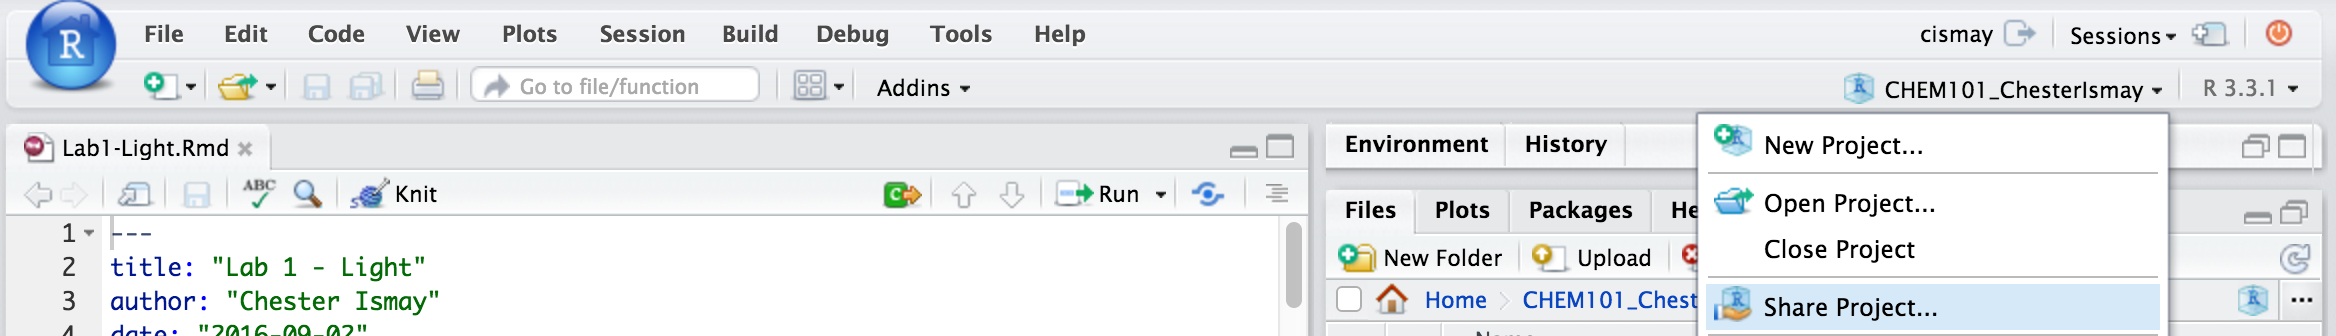
\includegraphics[width=\textwidth]{screenshots/shareproj1} \end{center}

\begin{center}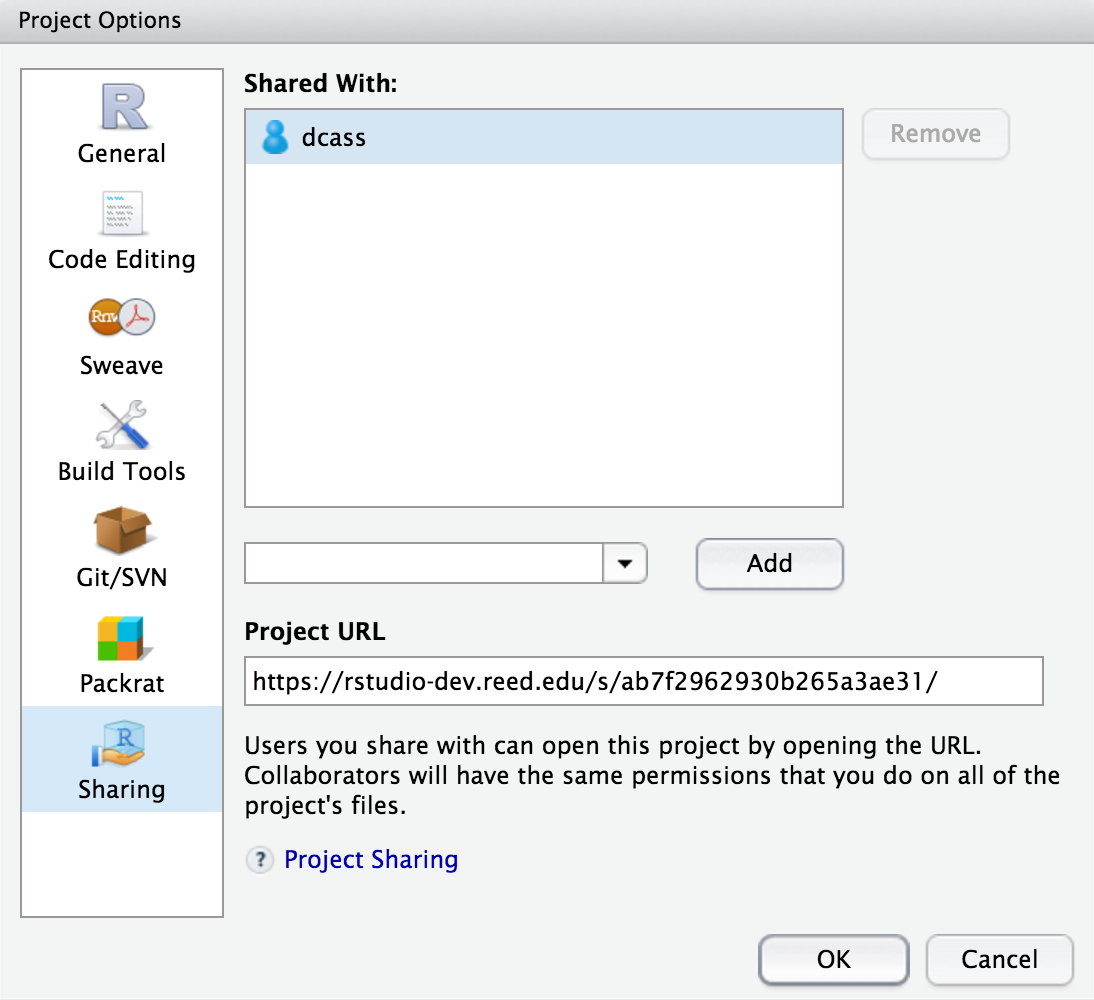
\includegraphics[width=0.6\linewidth]{screenshots/shareproj2} \end{center}

The link is given in the \textbf{Project URL}. Please copy this entire
link into the body of your emails to Danielle or I so that we can
quickly look into your errors.

\chapter{Lab 3: Reactor}\label{reactor}

\section{Getting the R Markdown lab
template}\label{getting-the-r-markdown-lab-template-1}

Begin by creating a new folder called \texttt{Lab3-Reactor} in your
\texttt{CHEM101\_FirstnameLastname} folder. Next, follow steps similar
to those found in the GIF in
\protect\hyperlink{getting-the-lab-template}{Section 1.1}, but select
the \textbf{Reactor} R Markdown template instead of \textbf{Light} and
save your file in the newly created \texttt{Lab3-Reactor} folder as
\texttt{lab3.Rmd}.

\section{The parts of the lab
template}\label{the-parts-of-the-lab-template-2}

\subsection{YAML}\label{yaml-1}

Refer back to \protect\hyperlink{the-yaml-header}{The YAML header}
section in Chapter \ref{light} for a review on what the entries here
mean. Remember to be careful with spacing!

\subsection{Initial R Chunk}\label{initial-r-chunk-2}

Remember that the \texttt{chemistr} package automatically loads in many
useful packages for you. It is loaded here in the \texttt{setup} chunk
and will need to be loaded in order to complete the plots in this lab.
It also includes functions such as \texttt{chem\_table} you worked with
in Lab 1 and \texttt{chem\_clustered.bar} and
\texttt{chem\_dual.scatter} that you will work with in this lab.

\subsection{Results chunk}\label{results-chunk}

Immediately after the \texttt{\#\#\ Results} header, you'll see a chunk
of code with name \texttt{chunk1} corresponding to your data from part
A. You will have three values for each of the four different shields you
used. Thus, the \texttt{material} variable will contain each of the
shields 3 times using the \texttt{c} function which \texttt{c}ombines
objects together and the \texttt{rep} function which \texttt{rep}eats
values a specified number of \texttt{times}. For each shield you'll have
a corresponding element value for each of the three elements. Thus, the
\texttt{element} vector is simply the three elements repeated 4
\texttt{times}. Lastly, you'll need to enter the \%T values in the
\texttt{value} variable. The last line creates a \texttt{data\_frame}
that has 12 rows and 3 columns. You are encouraged to enter
\texttt{View(shield\_data)} in the R console AFTER you have run this
chunk and the previous chunk. This will give you a glimpse into the
table layout of the data frame and also allow you to make changes to
your \texttt{value} entry as needed.

\subsection{Clustered bar graph chunk}\label{clustered-bar-graph-chunk}

In \texttt{chunk2}, you will be producing a bar graph that allows you to
look at how the different \texttt{element} values relate with the
different shielding values in terms of \%T. You also have the option to
change the colors you'd like to use by entering the names in quotation
marks in a \texttt{named\_colors} vector that is passed into the
\texttt{chem\_clustered.bar} function via the \texttt{colors} argument.
As noted in the R comments in \texttt{chunk2}, you can find a listing of
all of the named colors in R at
\textless{}\url{http://www.stat.columbia.edu/~tzheng/files/Rcolor.pdf}
\textgreater{}.

In the GIF below, I walk through the recommended steps to download and
save the template file in the appropriate location in your folder on the
RStudio Server. Additionally, you'll see what each of the different
variables correspond to in the \texttt{shield\_data} data frame and how
they are plotted in the clustered bar graph.

\vspace{0.1in}

\begin{center}\footnotesize{\url{https://raw.githubusercontent.com/ismayc/chemistr-book/master/gifs/cluster_bar.gif}}\end{center}

\vspace{0.1in}

As I have in the GIF, you should use the R Console to check your results
in the R chunks by either entering the R code line by line into the
Console or by pressing the \textbf{Run Current Chunk} button (the green
Play button). Additionally, you are encouraged to run all previous
chunks before running the current chunk by pressing the button just to
the left of the green Play button.

\subsection{Part B data entry}\label{part-b-data-entry}

In \texttt{chunk3} you'll enter data in much the same way as you did in
previous labs. Here you'll specify different values for
\texttt{thickness}, \texttt{abs}, and \texttt{trans}. Note here that
these are all numeric values and so you don't (AND SHOULDN'T) enter them
with quotes around them.

\subsection{Dual scatter plot}\label{dual-scatter-plot}

In \texttt{chunk4} you are presented with code to plot two vertical axis
numerical variables to go with one horizontal numerical variable. Here
we specify \texttt{thickness} as the horizontal and \texttt{abs} and
\texttt{trans} as the vertical axes. This should be an extension of the
work done in \protect\hyperlink{beers}{Lab 2} when you produced a
scatterplot via the \texttt{chem\_scatter} function.

\subsection{The remainder of the lab}\label{the-remainder-of-the-lab-2}

Lastly, you'll need to provide commentary text below the Discussion
header following the Exp 3 lab instructions.

\section{Note on white space}\label{note-on-white-space-2}

As you look over the R Markdown document you'll see that there is always
a new line of white space between the discussion and the R chunks and
also between each of the R chunks. It is highly recommended that you
also follow this workflow. You'll receive some strange errors at times
if you try to stack everything together and it's also much harder to
follow for another reader of your document if you have everything
bunched together. \textbf{White space is your friend!}

\section{Spell-check}\label{spell-check-2}

Just as I'm sure your English teachers have told you to spell check your
documents before submitting, you are also encouraged to do so here.
There is a built-in spell check option found near the \textbf{Knit}
button.

\begin{center}
\includegraphics[width=0.3\textwidth]{images/spellcheck} \end{center}

Please run this and carefully read over your lab report before
converting it to a PDF and submitting it to Moodle.

\section{Converting your Word document to
PDF}\label{converting-your-word-document-to-pdf-2}

The directions for each lab on Moodle say to upload a PDF version of
your lab. You'll see how to create this PDF from inside Microsoft Word
for Mac. A similar procedure can be done using LibreOffice
(\url{https://www.libreoffice.org/download/libreoffice-fresh/}) on
Linux, Mac, or Windows machines or Microsoft Word on a PC. You may also
have the option to \textbf{Save As} a PDF there and you can get to this
option by going to \textbf{File -\textgreater{} Save As -\textgreater{}
File Format: -\textgreater{} PDF} on the Mac if you prefer.

\vspace{0.1in}

\begin{center}\footnotesize{\url{https://raw.githubusercontent.com/ismayc/chemistr-book/master/gifs/word_pdf.gif}}\end{center}

\vspace{0.1in}

\section{Note on requesting help}\label{note-on-requesting-help-1}

It is extremely helpful for us if you can share a link to your RStudio
Project in any emails requesting help. This link is available by going
to your RStudio project in the top right corner of RStudio, clicking on
it and then selecting \textbf{Share Project}, and then select
\textbf{Sharing} as seen in the screenshots below.

\begin{center}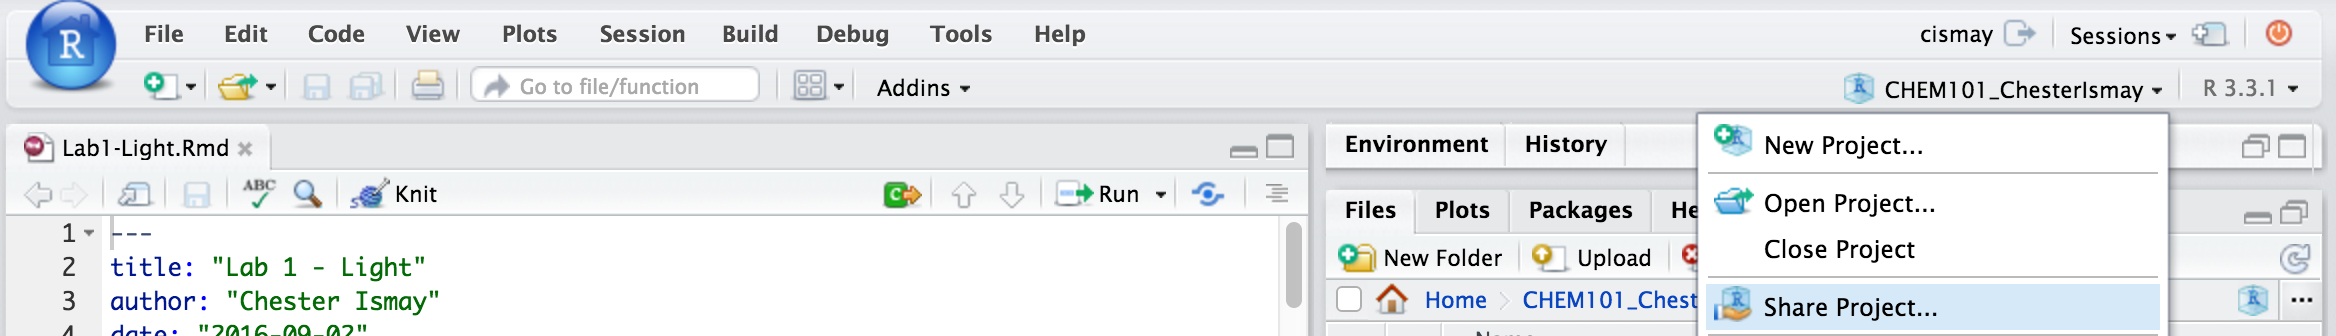
\includegraphics[width=\textwidth]{screenshots/shareproj1} \end{center}

\begin{center}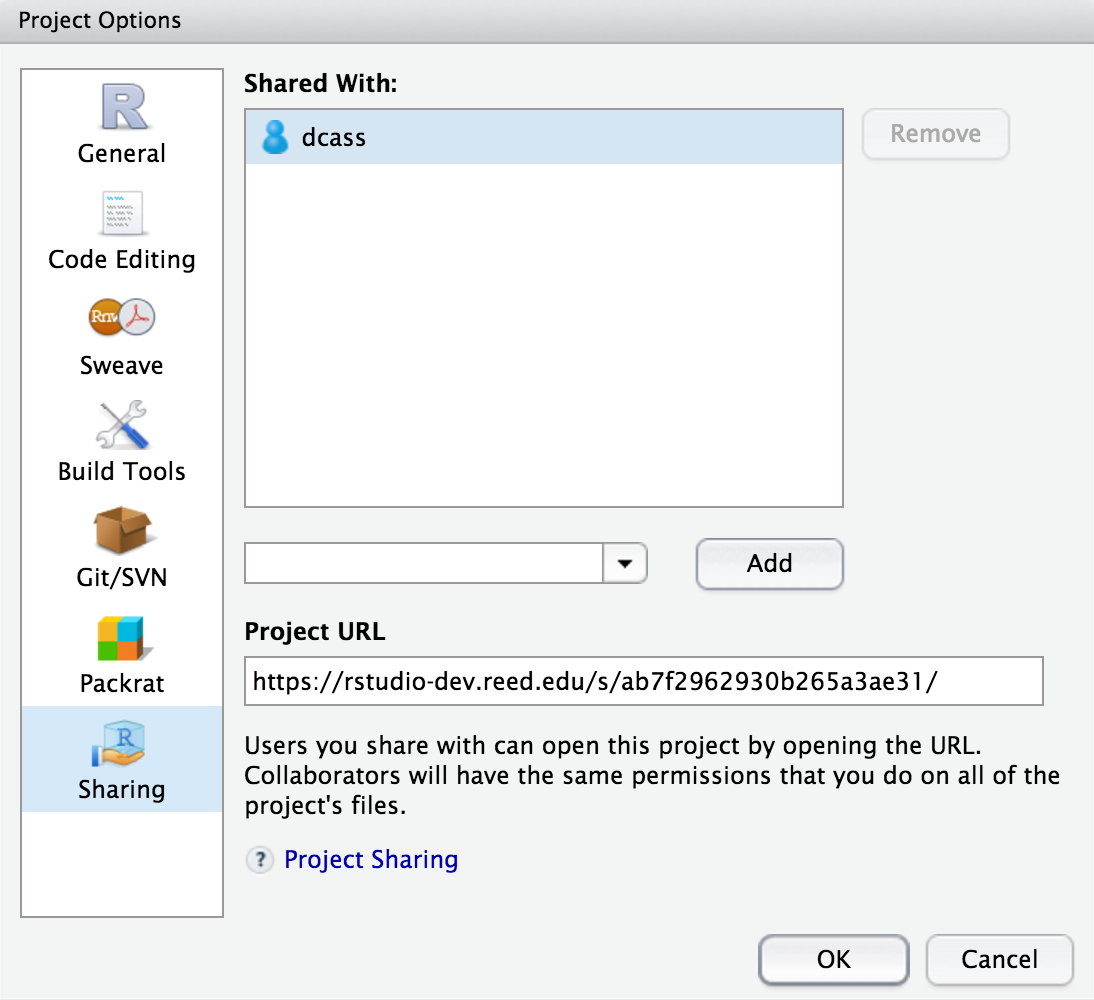
\includegraphics[width=0.6\linewidth]{screenshots/shareproj2} \end{center}

The link is given in the \textbf{Project URL}. Please copy this entire
link into the body of your emails to Danielle or I so that we can
quickly look into your errors.

\chapter{Lab 4: Iron}\label{iron}

\section{Getting the R Markdown lab
template}\label{getting-the-r-markdown-lab-template-2}

Begin by creating a new folder called \texttt{Lab4-Iron} in your
\texttt{CHEM101\_FirstnameLastname} folder. Next, follow steps similar
to those found in the GIF in
\protect\hyperlink{getting-the-lab-template}{Section 1.1}, but select
the \textbf{Iron Analysis} R Markdown template and save your file in the
newly created \texttt{Lab4-Iron} folder as \texttt{lab4.Rmd}.

\section{The parts of the lab
template}\label{the-parts-of-the-lab-template-3}

\subsection{YAML}\label{yaml-2}

Refer back to \protect\hyperlink{the-yaml-header}{The YAML header}
section in Chapter \ref{light} for a review on what the entries here
mean. Remember to be careful with spacing!

\subsection{Initial R Chunk}\label{initial-r-chunk-3}

Remember that the \texttt{chemistr} package automatically loads in many
useful packages for you. It is loaded here in the \texttt{setup} chunk
and will need to be loaded in order to complete the plots in this lab.

\subsection{Results chunk}\label{results-chunk-1}

As with previous labs, here you'll enter the values for \texttt{Iron}
and \texttt{Absorbance} and create a data frame named
\texttt{iron\_data} that pairs these two vectors together. Remember that
\texttt{Iron} and \texttt{Absorbance} must be of the same length (have
the same number of values) for the \texttt{data\_frame} function to
work.

\subsection{Plot chunk}\label{plot-chunk}

We are interested in fitting a linear regression line using
\texttt{Iron} as our predictor variable and \texttt{Absorbance} as our
response variable here. Make sure to add labels to your plots and
include an appropriate figure caption in the R chunk option
\texttt{fig.cap} following the guidelines in the commented R code in the
\texttt{plot1} chunk.

\subsection{Calculations}\label{calculations}

In this block of code you'll be doing some statistical calculations. If
you'd like to use R to do so, you'll need to first download the data
file from Moodle and read it into an object in R. So, for example, if
the data was saved as a CSV file called \texttt{iron\_class.csv}, you
could use the following code after you have Uploaded the file onto your
directory on the RStudio Server.

\begin{Shaded}
\begin{Highlighting}[]
\NormalTok{iron_class <-}\StringTok{ }\KeywordTok{read.csv}\NormalTok{(}\StringTok{"iron_class.csv"}\NormalTok{)}
\end{Highlighting}
\end{Shaded}

Now that you have the data read in, you can use the \texttt{group\_by},
\texttt{summarize}, and \texttt{mutate} functions in R to calculate
averages, standard deviations, and confidence intervals. If the name of
our iron variable for the class is \texttt{iron}, we can use the
\texttt{summarize} function to calculate the \textbf{mean} (average),
\textbf{standard deviation}, and \textbf{n} (how many values are in our
sample). We can then use the \texttt{mutate} function to create new
columns corresponding to the lower value of the confidence interval and
the upper value of the confidence interval:

\begin{Shaded}
\begin{Highlighting}[]
\NormalTok{iron_class %>%}
\StringTok{  }\KeywordTok{summarize}\NormalTok{(}\DataTypeTok{mean.iron =} \KeywordTok{mean}\NormalTok{(iron, }\DataTypeTok{na.rm =} \OtherTok{TRUE}\NormalTok{),}
            \DataTypeTok{sd.iron =} \KeywordTok{sd}\NormalTok{(iron, }\DataTypeTok{na.rm =} \OtherTok{TRUE}\NormalTok{),}
            \DataTypeTok{n.iron =} \KeywordTok{n}\NormalTok{()) %>%}
\StringTok{  }\KeywordTok{mutate}\NormalTok{(}\DataTypeTok{se.iron =} \NormalTok{sd.iron /}\StringTok{ }\KeywordTok{sqrt}\NormalTok{(n.iron),}
         \DataTypeTok{lower.ci.iron =} \NormalTok{mean.iron -}\StringTok{ }\KeywordTok{qt}\NormalTok{(}\DecValTok{1} \NormalTok{-}\StringTok{ }\NormalTok{(}\FloatTok{0.1} \NormalTok{/}\StringTok{ }\DecValTok{2}\NormalTok{), n.iron -}\StringTok{ }\DecValTok{1}\NormalTok{) *}\StringTok{ }\NormalTok{se.iron,}
         \DataTypeTok{upper.ci.iron =} \NormalTok{mean.iron +}\StringTok{ }\KeywordTok{qt}\NormalTok{(}\DecValTok{1} \NormalTok{-}\StringTok{ }\NormalTok{(}\FloatTok{0.1} \NormalTok{/}\StringTok{ }\DecValTok{2}\NormalTok{), n.iron -}\StringTok{ }\DecValTok{1}\NormalTok{) *}\StringTok{ }\NormalTok{se.iron)}
\end{Highlighting}
\end{Shaded}

To review, the \texttt{iron\_class} data frame is passed into the
\texttt{summarize} function, which creates three new variables
\texttt{mean.iron}, \texttt{sd.iron}, and \texttt{n.iron}. We need to
determine \texttt{n.iron} in order to calculate the standard error
denoted as \texttt{se.iron}. We can then put it all together to
calculate the confidence interval. Note here that instead of looking up
the values in the \(t\) table we can have R look them up for us at the
90\% level (this corresponds to the 95\textsuperscript{th} percentile
value in the \(t\) distribution with \texttt{n.iron\ -\ 1} degrees of
freedom).

\subsection{The remainder of the lab}\label{the-remainder-of-the-lab-3}

Lastly, you'll need to include a picture of your calculations if you
didn't use R and also a discussion of your results following the
directions in the template.

\section{Note on white space}\label{note-on-white-space-3}

As you look over the R Markdown document you'll see that there is always
a new line of white space between the discussion and the R chunks and
also between each of the R chunks. It is highly recommended that you
also follow this workflow. You'll receive some strange errors at times
if you try to stack everything together and it's also much harder to
follow for another reader of your document if you have everything
bunched together. \textbf{White space is your friend!}

\section{Spell-check}\label{spell-check-3}

Just as I'm sure your English teachers have told you to spell check your
documents before submitting, you are also encouraged to do so here.
There is a built-in spell check option found near the \textbf{Knit}
button.

\begin{center}
\includegraphics[width=0.3\textwidth]{images/spellcheck} \end{center}

Please run this and carefully read over your lab report before
converting it to a PDF and submitting it to Moodle.

\section{Converting your Word document to
PDF}\label{converting-your-word-document-to-pdf-3}

The directions for each lab on Moodle say to upload a PDF version of
your lab. You'll see how to create this PDF from inside Microsoft Word
for Mac. A similar procedure can be done using LibreOffice
(\url{https://www.libreoffice.org/download/libreoffice-fresh/}) on
Linux, Mac, or Windows machines or Microsoft Word on a PC. You may also
have the option to \textbf{Save As} a PDF there and you can get to this
option by going to \textbf{File -\textgreater{} Save As -\textgreater{}
File Format: -\textgreater{} PDF} on the Mac if you prefer.

\vspace{0.1in}

\begin{center}\footnotesize{\url{https://raw.githubusercontent.com/ismayc/chemistr-book/master/gifs/word_pdf.gif}}\end{center}

\vspace{0.1in}

\section{Note on requesting help}\label{note-on-requesting-help-2}

It is extremely helpful for us if you can share a link to your RStudio
Project in any emails requesting help. This link is available by going
to your RStudio project in the top right corner of RStudio, clicking on
it and then selecting \textbf{Share Project}, and then select
\textbf{Sharing} as seen in the screenshots below.

\begin{center}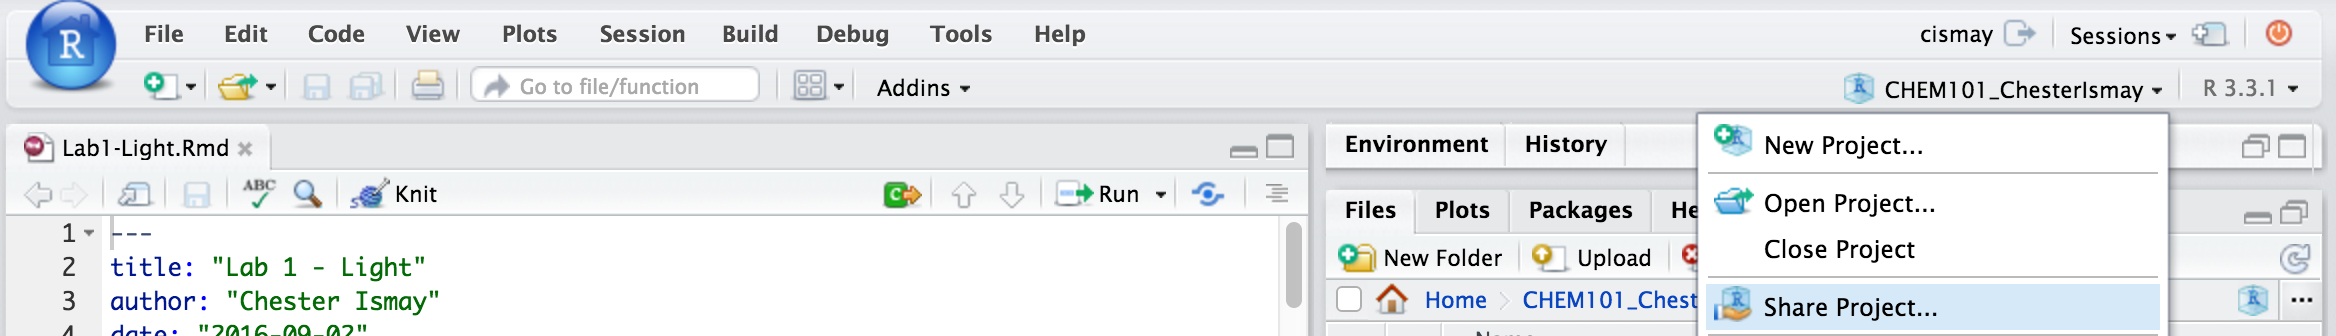
\includegraphics[width=\textwidth]{screenshots/shareproj1} \end{center}

\begin{center}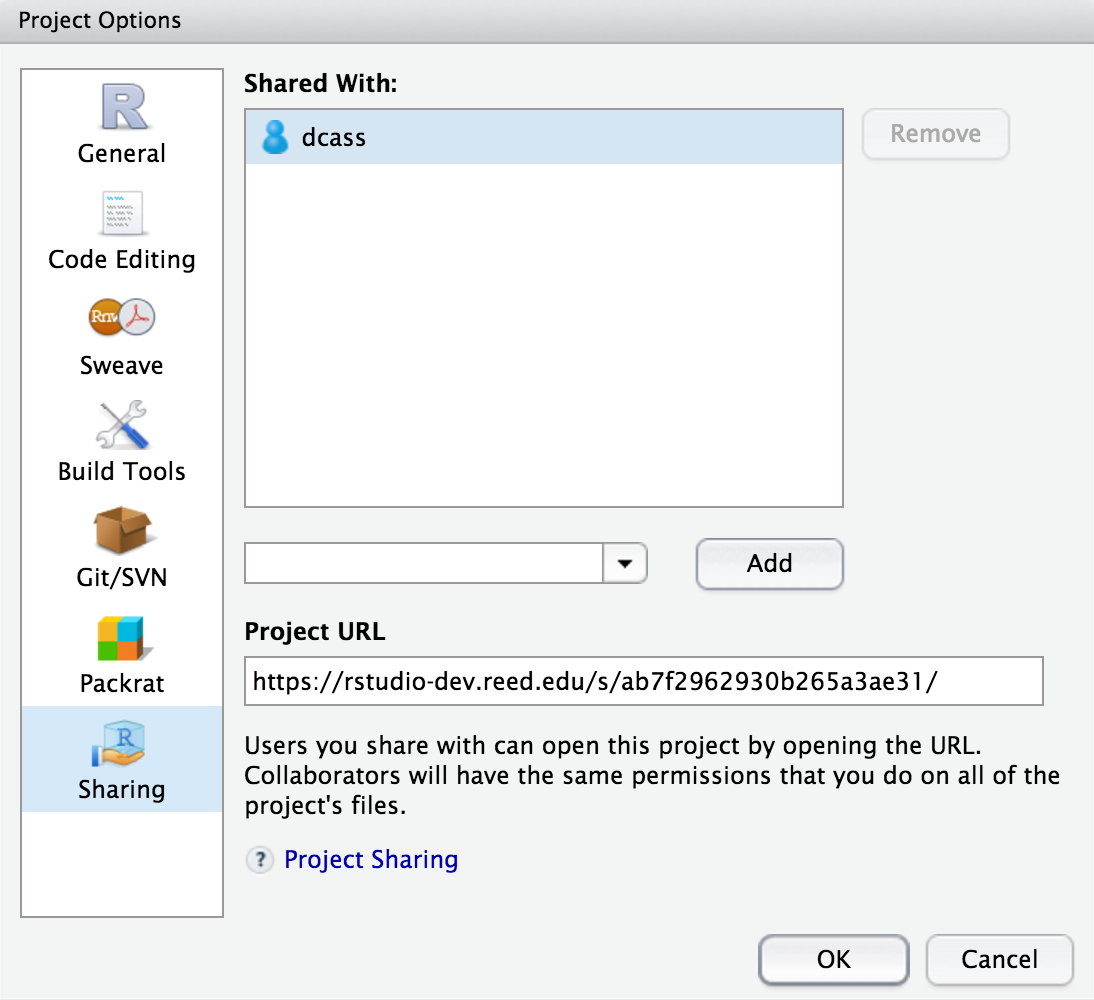
\includegraphics[width=0.6\linewidth]{screenshots/shareproj2} \end{center}

The link is given in the \textbf{Project URL}. Please copy this entire
link into the body of your emails to Danielle or I so that we can
quickly look into your errors.

\appendix


\chapter{RStudio Desktop}\label{rstudio-desktop}

More advanced users of RStudio may be interested in using the RStudio
Desktop version installed on their own computer instead of using the
RStudio Server. It is encouraged that all students do this after they
have some familiarity with how RStudio works. The RStudio Server is a
great way to learn how this works while providing the ability for more
advanced users to give support to learning through Shared Projects.
Downloading the RStudio Desktop allows for resources to be freed up on
the RStudio Server though and if you are performing more advanced
calculations it makes more sense to download your own version of RStudio
instead of running them on the RStudio Server.

\section{Downloading R and RStudio
Desktop}\label{downloading-r-and-rstudio-desktop}

It is worth noting that you can't just install RStudio Desktop without
installing R as RStudio needs to have R installed in order to run. A
step-by-step guide to installing R and RStudio Desktop with screenshots
can be found

\begin{itemize}
\tightlist
\item
  \href{http://www.reed.edu/data-at-reed/software/R/r_studio.html}{here}
  for the Mac and
\item
  \href{http://www.reed.edu/data-at-reed/software/R/r_studio_pc.html}{here}
  for a PC.
\end{itemize}

The process is a little more complicated for Linux machines, but
Googling ``RStudio for Linux'' wil likely lead you to some instructions.
Unless you plan to create PDF directly from R Markdown documents (which
requires a multiple gigabyte download of LaTeX) you can skip some of the
later steps of the installation guidelines.

\section{Downloading and installing
chemistr}\label{downloading-and-installing-chemistr}

I created the \texttt{chemistr} R package as a way to introduce students
of Chem 101/102 at Reed College to R without the sometimes intimidating
amounts of code needed to produce specific plots and tables. The package
also includes R Markdown lab report templates for each of the labs.

Intermediate users of R and RStudio may be used to using the
\texttt{install.packages} function to download and install R packages
from CRAN (The Comprehensive R Archive Network). This network is the
standard for R packages and, to be on CRAN, packages there go through a
series of tests to make sure they are working well. With the
\texttt{chemistr} package being developed recently (and still under
development), it does not currently reside on CRAN. But you can still
download a developmental version of it onto your machine running RStudio
Desktop.

\href{http://hadley.nz/}{Hadley Wickham} has created an R package called
\texttt{devtools} that allows for R packages to be more easily created
and shared with others. We will use this package to install the
\texttt{chemistr} package from my GitHub page. You'll need to enter
these commands into the R Console of your RStudio Desktop:

\begin{Shaded}
\begin{Highlighting}[]
\KeywordTok{install.packages}\NormalTok{(}\StringTok{"devtools"}\NormalTok{)}
\NormalTok{devtools::}\KeywordTok{install_github}\NormalTok{(}\StringTok{"ismayc/chemistr"}\NormalTok{)}
\end{Highlighting}
\end{Shaded}

After running these two commands you can check that \texttt{chemistr}
was installed correctly by entering \texttt{library(chemistr)} into the
R Console. If you get back to \texttt{\textgreater{}} without any error
messages, you should be good to go. Now you'll follow the same steps
given in each chapter of this book to get the R Markdown template for
that specific lab.

\begin{quote}
\textbf{File} -\textgreater{} \textbf{New File} -\textgreater{}
\textbf{R Markdown} -\textgreater{} \textbf{From Template}
-\textgreater{} NameOfLab
\end{quote}

You are encouraged to run the two lines of code above before you begin
each lab as there may have been slight corrections/changes made to the
lab templates. You can find a description of each change to the lab
templates
\href{https://github.com/ismayc/chemistr/blob/master/NEWS.md}{here} with
dates given.

\chapter{Lab 1: Light (More Details)}\label{appendix-light}

\section{\texorpdfstring{The \texttt{chem\_table}
function}{The chem\_table function}}\label{the-chem_table-function}

The \texttt{chem\_table} function is essentially a wrapper function to
the \texttt{pandoc.table} function in the \texttt{pander} package. Here
is the code for \texttt{chem\_table}:

\begin{Shaded}
\begin{Highlighting}[]
\NormalTok{chem_table <-}\StringTok{ }\NormalTok{function(data, caption)\{}
  \KeywordTok{names}\NormalTok{(data) <-}\StringTok{ }\KeywordTok{pandoc.strong.return}\NormalTok{(}\KeywordTok{names}\NormalTok{(data))}
  \KeywordTok{pandoc.table}\NormalTok{(data, }\DataTypeTok{caption =} \NormalTok{caption, }\DataTypeTok{style =} \StringTok{"multiline"}\NormalTok{,}
               \DataTypeTok{split.tables =} \OtherTok{Inf}\NormalTok{)}
  \KeywordTok{cat}\NormalTok{(}\StringTok{"}\CharTok{\textbackslash{}\textbackslash{}}\StringTok{newline"}\NormalTok{)}
\NormalTok{\}}
\end{Highlighting}
\end{Shaded}

We see here that \texttt{chem\_table} expects two arguments:

\begin{itemize}
\tightlist
\item
  \texttt{data} is a data frame containing the variables you'd like to
  appear in the table
\item
  \texttt{caption} is the caption we'd like to correspond to this table
\end{itemize}

Remember that you can run \texttt{?chemistr::chem\_table} to bring up
the help documentation for the function.

We first use the \texttt{pandoc.strong.return} function that bolds the
column names. We then call the \texttt{pandoc.table} function in the
\texttt{pander} package with \texttt{data} as our argument and then our
entered \texttt{caption} parameter as the \texttt{caption} argument to
\texttt{pandoc.table}. The last two argument for \texttt{style} and
\texttt{split.tables} are used to ensure the outputted table appears as
you might expect it to in the Word document:

\begin{itemize}
\item
  \texttt{style} set to \texttt{multiline} allow headers and table rows
  to span multiple lines of text. This may be helpful if you have long
  column names.
\item
  \texttt{split.tables} set to \texttt{Inf} ensures that wide tables
  will not be split into multiple tables.
\end{itemize}

Lastly, the \texttt{cat("\textbackslash{}\textbackslash{}newline")} code
specifies that an extra line of white space will be printed immediately
following the table.

\section{\texorpdfstring{The \texttt{include\_graphics}
function}{The include\_graphics function}}\label{the-include_graphics-function}

The \texttt{include\_graphics} function enables you to include pictures
that are stored as image files (\texttt{*.png} or \texttt{*.jpg}, for
example) into your Word document via R Markdown. It is a function in the
\texttt{knitr} package. If you'd like more information on how to use
\texttt{include\_graphics} run \texttt{?knitr::include\_graphics} in the
R Console. The important argument here is \texttt{path} which tells R
where to look for the file you want to include.

If you include your pictures in the same directory as your Rmd file you
need only specify the name of the file here in quotation marks. If you
have a \texttt{figure} folder in the same folder as your R Markdown
file, you'll need to specify that via something like:

\begin{Shaded}
\begin{Highlighting}[]
\NormalTok{knitr::}\KeywordTok{include_graphics}\NormalTok{(}\StringTok{"figure/myimage.png"}\NormalTok{)}
\end{Highlighting}
\end{Shaded}

Whatever you specify as the chunk option \texttt{fig.cap} will appear as
the figure caption. You are also encouraged to name the R chunk, which
will allow you to reference the figure later in your document as well as
automatic numbering of the figures:

\texttt{```\{r\ myimage,\ echo=FALSE,\ fig.cap="Here\ is\ my\ picture"\}}

\texttt{knitr::include\_graphics("figure/myimage.png")}

\texttt{```}

We could then reference our picture in the text of our document by using
\texttt{\textbackslash{}@ref(fig:myimage)}.

\renewcommand{\bibname}{References}
\addcontentsline{toc}{chapter}{References}
\bibliography{bib/packages.bib,bib/books.bib,bib/articles.bib}
% 
% 

\end{document}
